\documentclass{article}
\usepackage[T1]{fontenc}
\usepackage[utf8]{inputenc}
\usepackage[portuguese]{babel}

\title{Lista 5 \\
\large Introdução à Análise Numérica \\
Solução numérica de EDP}
\author{Lucas Emanuel Resck Domingues}
\date{\today}

\usepackage{natbib}
\usepackage{graphicx}
\usepackage{amsmath}
\usepackage{listings}
\usepackage{multirow}
\usepackage{hyperref}
\usepackage{amsfonts}

% \lstset{columns=fullflexible}

% Hyperlinks
\usepackage{hyperref}
\hypersetup{
    colorlinks=true,
    allcolors=,  % Nothing change colors
    urlcolor=blue  % URL changes color
}

\begin{document}

    \maketitle

    Esta é a solução da questão 7.

    \begin{itemize}
        \item[(a)] O método CTCS para a equação da onda
            descrita foi implementado em Matlab e pode
            ser conferido no Apêndice \ref{appendix:ctcs}.

            O algoritmo particiona $[-10, 10]$ com intervalo
            $\Delta x$ desejado e $[0, T]$ com intervalo
            $\Delta t$ desejado. Então calcula-se $u_0$ utilizando a função
            $f(x) = e^{-x^2}$, a matriz $A$ utilizando
            $\sigma = c \Delta t / \Delta x = \Delta t / \Delta x$
            (dado que $c = 1$) e,
            finalmente, $u_1$, utilizando $u_0$, $g(x) = 0$, $p(x) = 0$
            e $q(x) = 0$. Dado que temos as condições iniciais,
            podemos partir para a iteração de $u_i$ para obter
            o valor de $u$ em todo o \textit{grid}. Isso ocorre com
            a seguinte iteração (que é autoexplicativa):

            \begin{lstlisting}[language=Matlab]
aux = zeros(m, 1);
aux(1) = sigma^2*p(i*dt);
aux(end) = sigma^2*q(i*dt);
u(1:end, i+1) = A*u(1:end, i) - u(1:end, i-1) + aux;
            \end{lstlisting}

            A construção do gráfico ocorre utilizando a função
            \lstinline[language=Matlab]{surf}. Antes da exibição do gráfico,
            é realizada uma diminuição da quantidade de pontos, amostrando
            apenas alguns deles, igualmente espaçados. Observe que isso
            não impacta o cálculo de $u$, afinal é apenas no momento da
            visualização que isso ocorre. Note que isso é necessário,
            pois são muitos pontos que impossibilitam a correta visualização
            da solução numérica $u$.

            A Figura \ref{fig:wave_1} mostra o resultado do método CTCS
            para $\Delta x = 0.04$ e $\Delta t = 0.02$ em
            $[-10, 10] \times [0, 120]$. Observamos que a onda inicial se divide
            em duas ondas menores, até que essas duas ondas ``rebatem'' na ``parede''
            (condição de fronteira) e invertem. Depois elas se encontram novamente,
            dessa vez invertidas, logo
            se separaram, invertem e de juntam novamente, exatamente como a condição
            inicial.

            \begin{figure}[!h]
                \centerline{
                    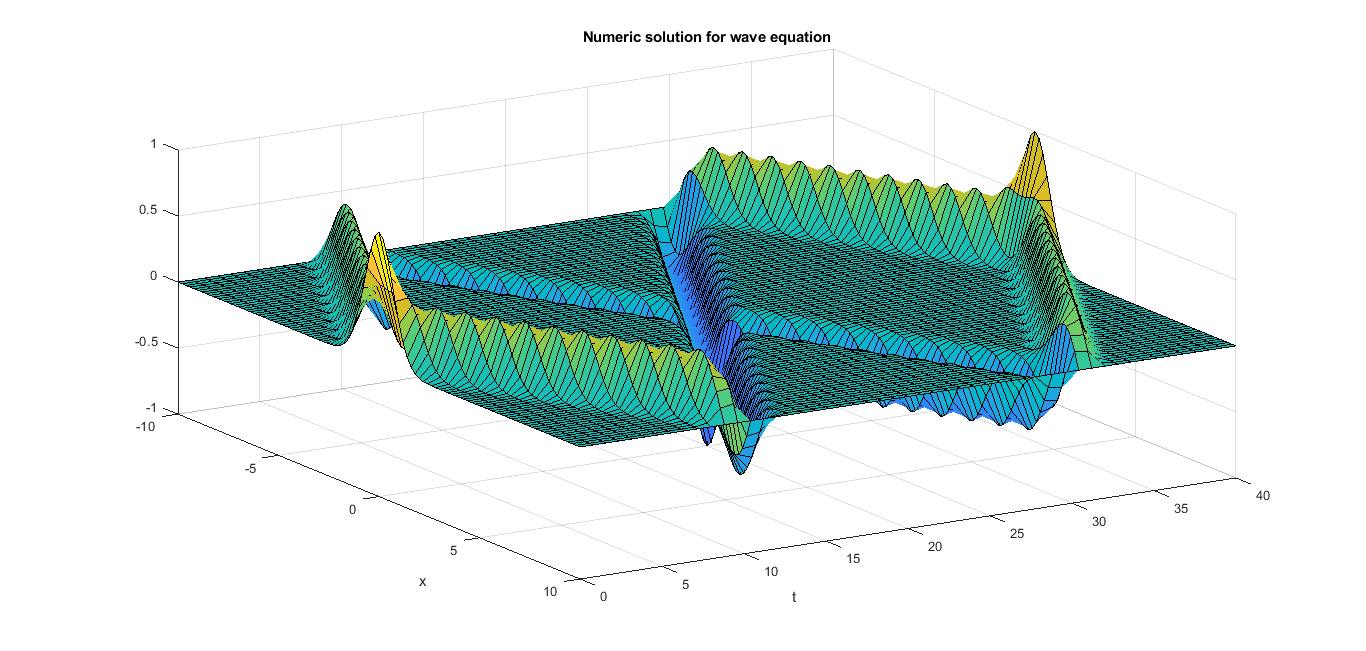
\includegraphics[width=1.4\textwidth]{images/wave_1.png}
                }
                \caption{Solução numérica CTCS para a equação da onda, com $c = 1$,
                $\Delta x = 0.04$ e $\Delta t = 0.02$, na região $[-10, 10] \times [0, 40]$.}
                \label{fig:wave_1}
            \end{figure}

            \clearpage

        \item[(b)] As Figuras \ref{fig:wave_2} e \ref{fig:wave_3} mostram
            o resultado da solução numérica nas regiões
            $[-10, 10] \times [0, 80]$ e $[-10, 10] \times [0, 120]$,
            respectivamente.

            Fica clara a repetição do padrão que é descrito na Figura
            \ref{fig:wave_1}. Esse padrão se repete 2 vezes na Figura \ref{fig:wave_2}
            e 3 vezes na Figura \ref{fig:wave_3}.

            \begin{figure}[!h]
                \centerline{
                    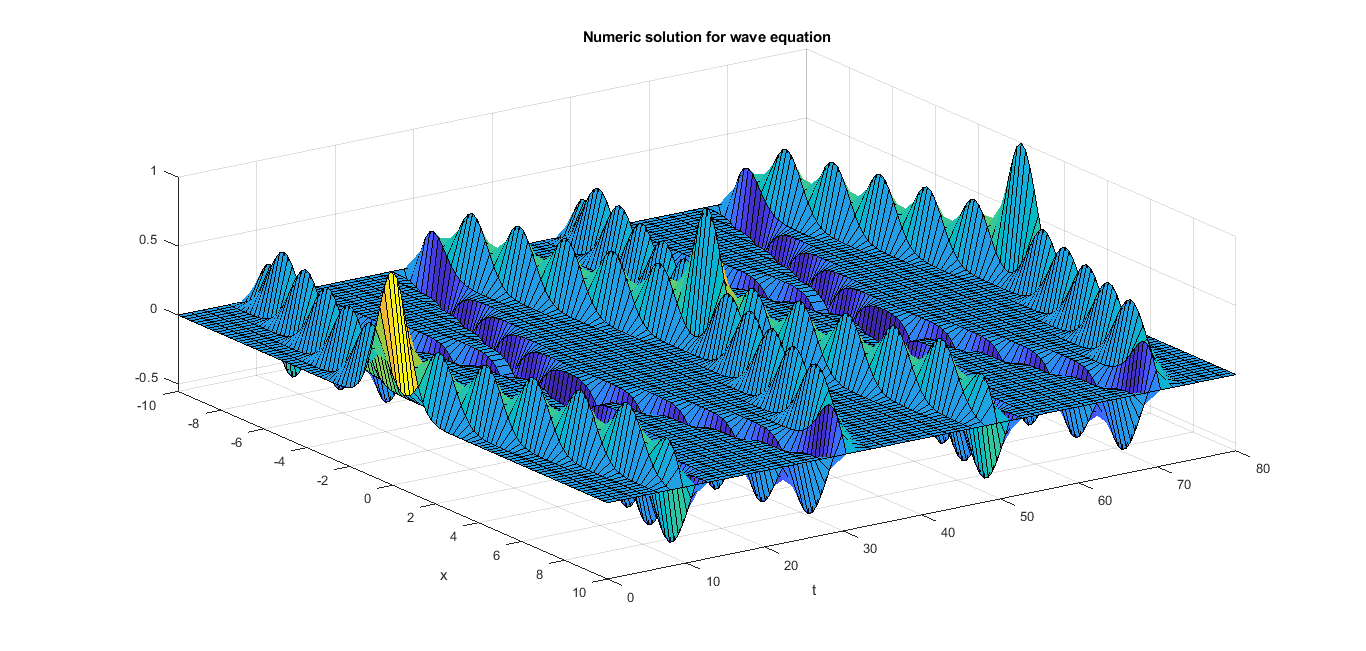
\includegraphics[width=1.4\textwidth]{images/wave_2.png}
                }
                \caption{Solução numérica CTCS para a equação da onda, com $c = 1$,
                $\Delta x = 0.04$ e $\Delta t = 0.02$, na região $[-10, 10] \times [0, 80]$.}
                \label{fig:wave_2}
            \end{figure}

            \begin{figure}[!h]
                \centerline{
                    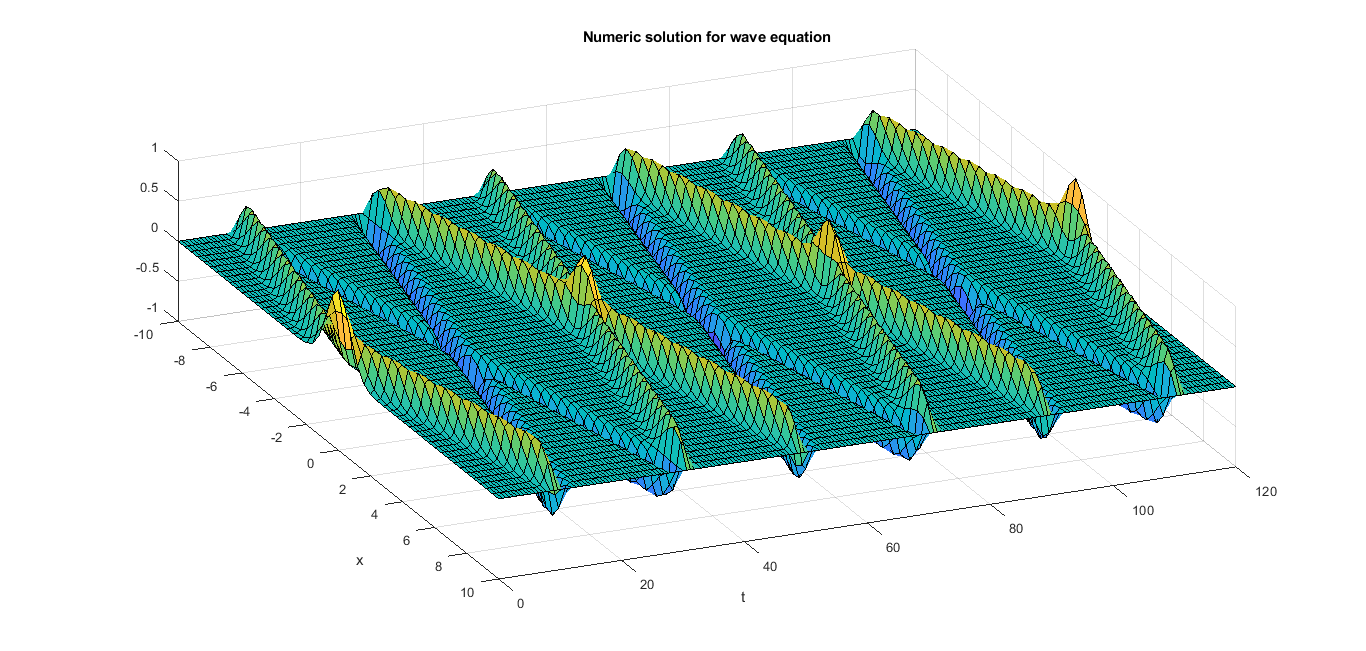
\includegraphics[width=1.4\textwidth]{images/wave_3.png}
                }
                \caption{Solução numérica CTCS para a equação da onda, com $c = 1$,
                $\Delta x = 0.04$ e $\Delta t = 0.02$, na região $[-10, 10] \times [0, 120]$.}
                \label{fig:wave_3}
            \end{figure}

            \clearpage

        \item[(c)] A condição CFL foi obedecida em todos os exemplos anteriores.
            Vamos, agora, violar essa condição. Vamos escolher $\Delta x = 0.4$
            e $\Delta t = 0.040008$. Ou seja,

            $$\sigma = c\dfrac{\Delta t}{\Delta x} = \dfrac{0.040008}{0.4} > 1$$

            Os valores foram escolhidos para que $\sigma > 1$.

            A Figura \ref{fig:wave_4} apresenta o resultado da solução
            numérica CTCS para $\Delta x = 0.04$ e $\Delta t = 0.040008$ em
            $[-10, 10] \times [0, 40]$. Observamos que a solução começa a
            ``explodir''. Note que esse valor curioso para $\Delta t$ foi
            escolhido cuidadosamente de modo que fosse possível
            visualizar tanto a onda quanto a ``explosão''.

            \begin{figure}[!h]
                \centerline{
                    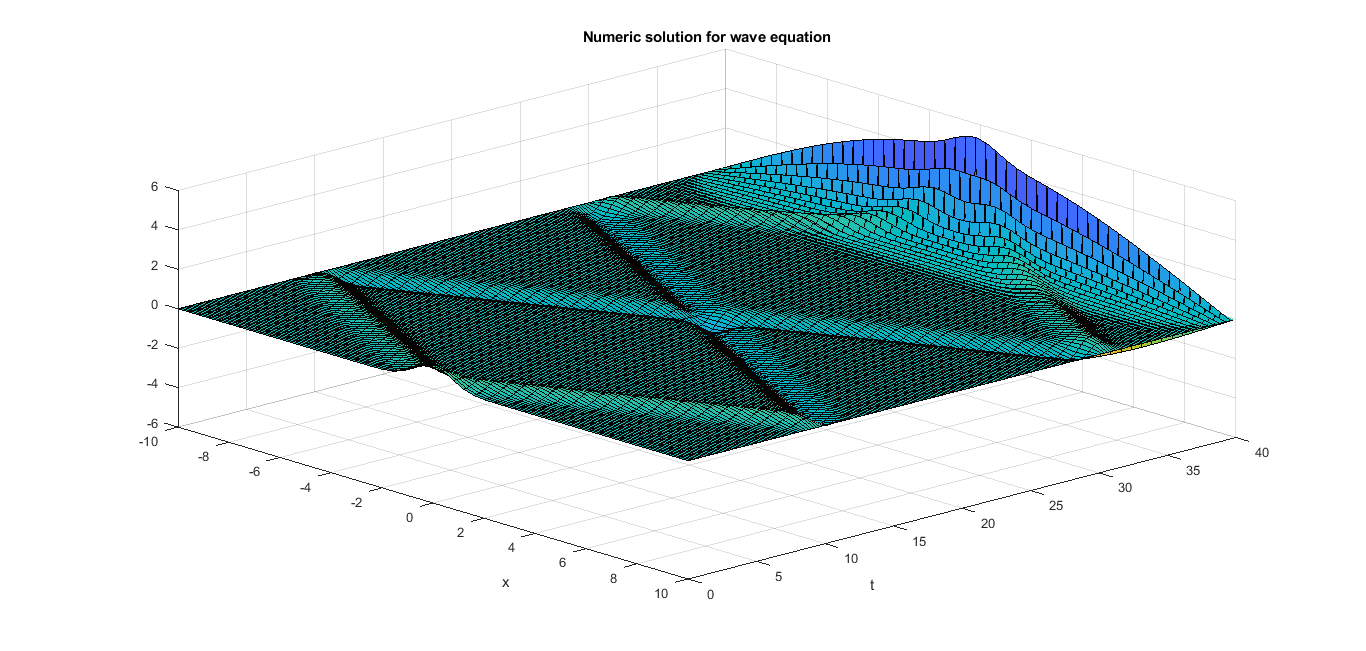
\includegraphics[width=1.4\textwidth]{images/wave_4.png}
                }
                \caption{Solução numérica CTCS para a equação da onda, com $c = 1$,
                $\Delta x = 0.04$ e $\Delta t = 0.040008$, na região $[-10, 10] \times [0, 40]$.}
                \label{fig:wave_4}
            \end{figure}

            \clearpage

            A Figura \ref{fig:wave_5} mostra o resultado para um valor de
            $\Delta t$, digamos, menos generoso: $\Delta t = 0.041$. A explosão
            chega à ordem de grandeza $10^{170}$!

            \begin{figure}[!h]
                \centerline{
                    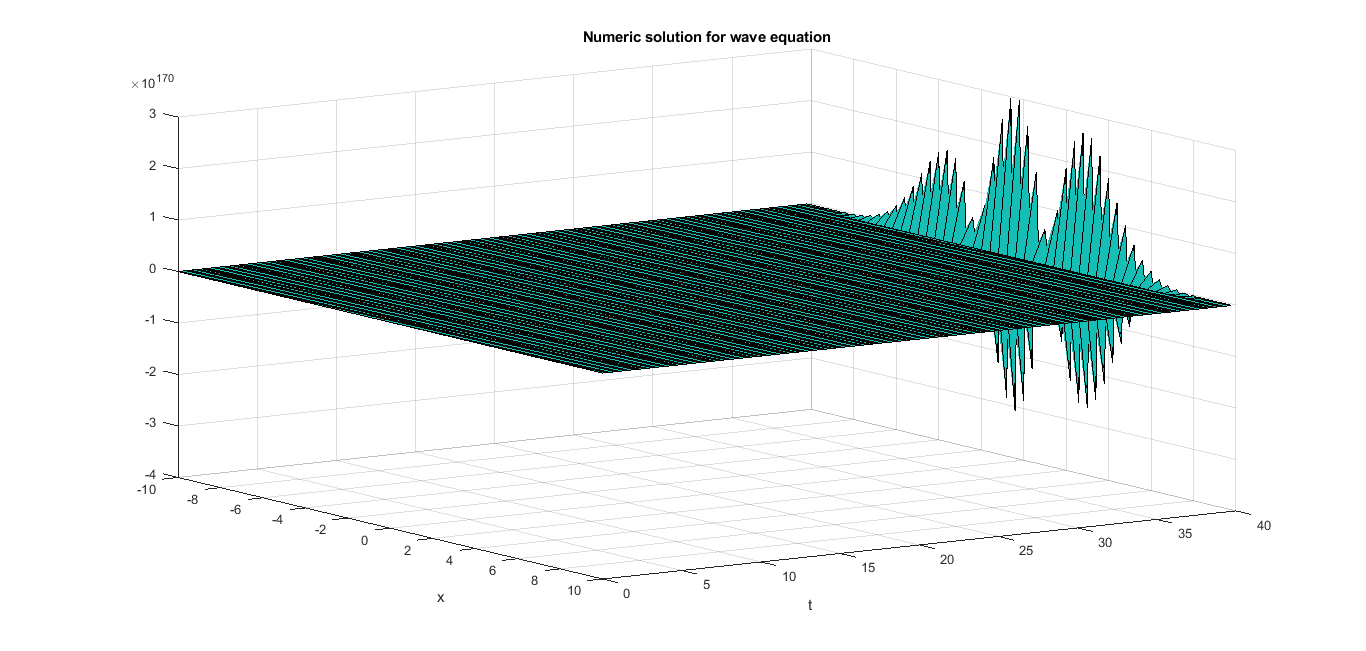
\includegraphics[width=1.4\textwidth]{images/wave_5.png}
                }
                \caption{Solução numérica CTCS para a equação da onda, com $c = 1$,
                $\Delta x = 0.04$ e $\Delta t = 0.041$, na região $[-10, 10] \times [0, 40]$.}
                \label{fig:wave_5}
            \end{figure}


    \end{itemize}

    \clearpage

    \appendix

    \section{Método CTCS para a equação da onda}
        \label{appendix:ctcs}

\end{document}
